% Options for packages loaded elsewhere
\PassOptionsToPackage{unicode,backref,colorlinks=true}{hyperref}
\PassOptionsToPackage{hyphens}{url}
%
\documentclass[
  10pt,
  a4paper,
]{article}
\usepackage{amsmath,amssymb}
\usepackage[]{tgpagella}
\usepackage{ifxetex,ifluatex}
\ifnum 0\ifxetex 1\fi\ifluatex 1\fi=0 % if pdftex
  \usepackage[T1]{fontenc}
  \usepackage[utf8]{inputenc}
  \usepackage{textcomp} % provide euro and other symbols
\else % if luatex or xetex
  \usepackage{unicode-math}
  \defaultfontfeatures{Scale=MatchLowercase}
  \defaultfontfeatures[\rmfamily]{Ligatures=TeX,Scale=1}
\fi
% Use upquote if available, for straight quotes in verbatim environments
\IfFileExists{upquote.sty}{\usepackage{upquote}}{}
\IfFileExists{microtype.sty}{% use microtype if available
  \usepackage[]{microtype}
  \UseMicrotypeSet[protrusion]{basicmath} % disable protrusion for tt fonts
}{}
\makeatletter
\@ifundefined{KOMAClassName}{% if non-KOMA class
  \IfFileExists{parskip.sty}{%
    \usepackage{parskip}
  }{% else
    \setlength{\parindent}{0pt}
    \setlength{\parskip}{6pt plus 2pt minus 1pt}}
}{% if KOMA class
  \KOMAoptions{parskip=half}}
\makeatother
\usepackage{xcolor}
\IfFileExists{xurl.sty}{\usepackage{xurl}}{} % add URL line breaks if available
\IfFileExists{bookmark.sty}{\usepackage{bookmark}}{\usepackage{hyperref}}
\hypersetup{
  pdftitle={Submodels, priors, and pooling the link parameters in the survival example},
  pdfauthor={Andrew Manderson},
  hidelinks,
  pdfcreator={LaTeX via pandoc}}
\urlstyle{same} % disable monospaced font for URLs
\usepackage[margin=2.25cm]{geometry}
\usepackage{graphicx}
\makeatletter
\def\maxwidth{\ifdim\Gin@nat@width>\linewidth\linewidth\else\Gin@nat@width\fi}
\def\maxheight{\ifdim\Gin@nat@height>\textheight\textheight\else\Gin@nat@height\fi}
\makeatother
% Scale images if necessary, so that they will not overflow the page
% margins by default, and it is still possible to overwrite the defaults
% using explicit options in \includegraphics[width, height, ...]{}
\setkeys{Gin}{width=\maxwidth,height=\maxheight,keepaspectratio}
% Set default figure placement to htbp
\makeatletter
\def\fps@figure{htbp}
\makeatother
\setlength{\emergencystretch}{3em} % prevent overfull lines
\providecommand{\tightlist}{%
  \setlength{\itemsep}{0pt}\setlength{\parskip}{0pt}}
\setcounter{secnumdepth}{5}
\usepackage{amsmath}
% I always seem to need tikz for something
\usepackage{tikz}
\usetikzlibrary{positioning, shapes, intersections, through, backgrounds, fit, decorations.pathmorphing, angles, quotes}
\usepackage{lineno}
% \linenumbers


\makeatletter
\@ifclassloaded{imsart}{}{
\usepackage{setspace}
\onehalfspacing
}
\makeatother

\usepackage{relsize}
\usepackage{placeins}

% required for landscape pages. beware, they back the build very slow.
\usepackage{pdflscape}

% table - `gt' package uses these, often unimportant
\usepackage{longtable}
\usepackage{booktabs}
\usepackage{caption}

\usepackage{color}
\definecolor{myredhighlight}{RGB}{180, 15, 32}
\definecolor{mydarkblue}{RGB}{0, 33, 79}
\definecolor{mymidblue}{RGB}{44, 127, 184}
\definecolor{mylightblue}{RGB}{166, 233, 255}

\usepackage{colortbl}

\newcommand{\semitransp}[2][35]{\color{fg!#1}#2}

\setcounter{secnumdepth}{3}

\let\Oldcap\cap
\renewcommand{\cap}{\mathrel{\mathsmaller{\Oldcap}}}

% pd stands for: probability distribution and is useful to distringuish
% marignals for probabilities specifically p(p_{1}) and the like.
\newcommand{\pd}{\text{p}}
\newcommand{\q}{\text{q}}
\newcommand{\w}{\text{w}}
\newcommand{\pdr}{\text{r}}
\newcommand{\pdrh}{\hat{\text{r}}}

% melding
\newcommand{\ppoolphi}{\pd_{\text{pool}}(\phi)}
\newcommand{\pmeld}{\pd_{\text{meld}}}

% the q(x)w(x), "weighted target" density 
% for the moment I'm going to call it s(x), as that is the next letter of the 
% alphabet. Can change it later
\newcommand{\s}{\text{s}}
% direct density estimate - replaces lambda.
\newcommand{\ddest}{\text{s}}
% target weighting function
\newcommand{\tarw}{\text{u}}

% constants - usually sizes of things
\newcommand{\Nx}{N}
\newcommand{\Nnu}{\text{N}_{\text{nu}}}
\newcommand{\Nde}{\text{N}_{\text{de}}}
\newcommand{\Nmc}{\text{N}_{\text{mc}}}
\newcommand{\Nw}{W}
\newcommand{\Nm}{M}
\newcommand{\Ns}{S}
\newcommand{\Np}{P}

% locales - could switch to x and x'
\newcommand{\xnu}{x_{\text{nu}}}
\newcommand{\xde}{x_{\text{de}}}
\newcommand{\phinu}{\phi_{\text{nu}}}
\newcommand{\phide}{\phi_{\text{de}}}

% sugiyama stuff
\newcommand{\pdnu}{\pd_{\text{nu}}}
\newcommand{\pdde}{\pd_{\text{de}}}

% indices 
\newcommand{\wfindex}{w}
\newcommand{\sampleindex}{n}
\newcommand{\modelindex}{m}
\newcommand{\stageindex}{s}
\newcommand{\phiindex}{p}

% independence symbol
\newcommand{\indep}{\perp\!\!\!\perp}
\newcommand{\setcomp}{\mathsf{c}}

\newtheorem{theorem}{Theorem}[section]
\newtheorem{corollary}{Corollary}[theorem]

\DeclareMathOperator*{\argmin}{arg\,min}

% ARDS example in text commands
\newcommand{\paoii}{PaO\textsubscript{2}}
\newcommand{\fioii}{FiO\textsubscript{2}}
\newcommand{\spoii}{SpO\textsubscript{2}}
\newcommand{\pfratio}{\paoii/\fioii}
\newcommand{\sfratio}{\spoii/\fioii}
\ifluatex
  \usepackage{selnolig}  % disable illegal ligatures
\fi
\newlength{\cslhangindent}
\setlength{\cslhangindent}{1.5em}
\newlength{\csllabelwidth}
\setlength{\csllabelwidth}{3em}
\newenvironment{CSLReferences}[2] % #1 hanging-ident, #2 entry spacing
 {% don't indent paragraphs
  \setlength{\parindent}{0pt}
  % turn on hanging indent if param 1 is 1
  \ifodd #1 \everypar{\setlength{\hangindent}{\cslhangindent}}\ignorespaces\fi
  % set entry spacing
  \ifnum #2 > 0
  \setlength{\parskip}{#2\baselineskip}
  \fi
 }%
 {}
\usepackage{calc}
\newcommand{\CSLBlock}[1]{#1\hfill\break}
\newcommand{\CSLLeftMargin}[1]{\parbox[t]{\csllabelwidth}{#1}}
\newcommand{\CSLRightInline}[1]{\parbox[t]{\linewidth - \csllabelwidth}{#1}\break}
\newcommand{\CSLIndent}[1]{\hspace{\cslhangindent}#1}

\title{Submodels, priors, and pooling the link parameters in the
survival example}
\author{Andrew Manderson}
\date{25 June, 2021}

\begin{document}
\maketitle

\hypertarget{models}{%
\section{Models}\label{models}}

There are \(i = 1, \ldots, N\) individuals (icustays) in the data set.
Each individual is admitted to the ICU at time \(0\), and is discharged
or dies at time \(C_{i}\). See appendix \ref{cohort-selection-criteria}
for information on \(N\) and how the individuals were selected from
MIMIC-III.

\hypertarget{pf-ratio-model-b-spline-pd_1}{%
\subsection{\texorpdfstring{P/F ratio model (B-spline):
\(\pd_{1}\)}{P/F ratio model (B-spline): \textbackslash pd\_\{1\}}}\label{pf-ratio-model-b-spline-pd_1}}

Each individual has P/F ratio observations \(z_{i, j}\) at times
\(t_{i, j}\), with \(j = 1, \ldots, J_{i}\). For each individual denote
the vector of observations
\(\boldsymbol{z}_{i} = (z_{i, 1}, \ldots, z_{i, J_{i}})\) and
observation times
\(\boldsymbol{t}_{i} = (t_{i, 1}, \ldots, t_{i, J_{i}})\). To improve
computational performance, we standardise the P/F data for each
individual such that
\(z_{i, j} = \frac{\tilde{z}_{i, j} - \overline{z}_{i}}{\hat{s}_{i}}\),
where \(\tilde{z}_{i, j}\) is the underlying unstandardised observation
with mean \(\overline{z}_{i}\) and standard deviation \(\hat{s}_{i}\).
Similarly we rescale the threshold for respiratory failure:
\(\tau_{i} = \frac{300 - \overline{z}_{i}}{\hat{s}_{i}}\).

We choose to model the P/F ratio using a B-spline of degree 3, with 2
boundary knots and 7 internal knots, and do not include an intercept
column in the spline basis. The internal knots are evenly spaced between
the two boundary knots at \(\min(\boldsymbol{t_{i}})\) and
\(\max(\boldsymbol{t_{i}})\). These choices result in
\(k = 1, \ldots, 10\) spline basis terms per individual, with
coefficients \(\zeta_{i, k}\) where
\(\boldsymbol{\zeta}_{i} = (\zeta_{i, 1}, \ldots, \zeta_{i, 10})\). We
denote the individual specific B-spline basis evaluated at time
\(t_{i, j}\) as \(B_{i}(t_{i, j}) \in \mathbb{R}_{+} \cup \{0\}\) so
that the submodel can be written as \begin{equation}
  z_{i, j} = \beta_{0, i} + B_{i}(t_{i, j})\boldsymbol{\zeta}_{i} + \varepsilon_{i, j}
\end{equation} We employ a weakly informative prior for the intercept,
and a heavy tailed (\(t_{5}\)) distribution for the error
term\footnote{P/F data contain many outliers for, amongst many possible
  reasons, arterial/venous blood sample mis-labelling; incorrectly
  recorded oxygenation support information; and differences between
  sample collection time, lab result time, and the observation time
  recorded as in the EHR.} with a weakly informative half-normal prior
for unknown scale parameter \begin{equation}
  \beta_{0, i} \sim \text{N}(0, 1^2), \,\, \varepsilon_{i, j} \sim t_{5}(0, \omega), \,\,  \omega \sim \text{N}_{+}(0, 1^2).
\end{equation} For the spline basis coefficients we set
\(\zeta_{i, 1} \sim \text{N}(0, 0.5^2)\), and for \(k = 2, \ldots, 10\)
we employ a random-walk prior
\(\zeta_{i, k} \sim \text{N}(\zeta_{i, k - 1}, 0.5^2)\).

If a solution to the following optimisation problem exists, then we
conclude that a respiratory failure event \(d_{i} = 1\) occurred at
event time \(T_{i}\). \begin{equation}
  T_{i} = \min_{t} \left\{
    \tau_{i} = \beta_{0, i} + B_{i}(t)\boldsymbol{\zeta}_{i}
    \mid
    t \in [\max(0, \min(\boldsymbol{t_{i}})), \max(\boldsymbol{t_{i}})]
  \right\},
  \label{eqn:event_time_model_def}
\end{equation} We use a standard multiple root finder
(\protect\hyperlink{ref-soetaert_rootsolve_2020}{Soetaert \emph{et al.},
2020}) to obtain a solution. If there are no roots then the individual
died or was discharged before respiratory failure occurred so we set
\(T_{i} = C_{i}\) and \(d_{i} = 0\).

We would like to link this submodel with the other submodels via
\((\{T_{i}, d_{i}\}_{i = 1}^{N})\). However, care is required when
defining the link parameter \(\phi_{1 \cap 2}\) as it is a deterministic
function of \((\beta_{0, i}, \boldsymbol{\zeta}_{i})\). Keeping with the
notation of \protect\hyperlink{ref-goudie_joining_2019}{Goudie \emph{et
al.}} (\protect\hyperlink{ref-goudie_joining_2019}{2019}), we define
\(\theta_{1, i} = (\beta_{0, i}, \boldsymbol{\zeta}_{i})\), with
\(\phi_{1 \cap 2, i} = f(\theta_{1, i}) = (T_{i}, d_{i})\), where \(f\)
is the solution to \eqref{eqn:event_time_model_def}, and
\(\phi_{1 \cap 2} = \phi_{1 \cap 2}(\theta_{1}) = (f(\theta_{1, i}), \ldots, f(\theta_{1, N}))\).
It is also convenient to define
\(\theta_{1} = (\theta_{1, 1}, \ldots, \theta_{1, N})\).

Care is also require when considering the prior marginal
\(\pd_{1}(\phi_{1 \cap 2})\). We note that
\(\pd_{1}(\phi_{1 \cap 2}) = \prod_{i = 1}^{N}\pd_{1, i}(T_{i}, d_{i})\),
and that \(\pd_{1, i}(T_{i}, d_{i})\) conditions on each individual's
length of stay (in specifying the location of the knots), as well as the
range, mean, and standard deviation of the P/F data (by standardising
\(\tilde{z}_{i, j}\)). The analytic form of \(\pd_{1, i}(T_{i}, d_{i})\)
is not available and must be estimated, which we discuss in Section
\ref{estimating-submodel-prior-marginal-distributions}. To completely
align with our chained melding notation we also define
\(Y_{1} = (\{\boldsymbol{z}_{i}, \boldsymbol{t}_{i}\}_{i = 1}^{N})\) and
\(\psi_{1} = \omega\).

Figure \ref{fig:pf_fit_and_fluid_fit_plot} displays the P/F data, the
fitted submodel, and derived event times for individuals \(i = 6, 13\),
and \(15\). The spline appears to fit the raw P/F data well, with the
heavy tailed error term accounting for the larger deviations away from
the fitted value. It is interesting to see the relatively wide,
multimodal distribution for \(\{T_{13}, d_{13}\}\) (and for some other
individuals not shown here).

\hypertarget{cumulative-fluid-model-piecewise-linear-pd_3}{%
\subsection{\texorpdfstring{Cumulative fluid model (piecewise linear)
\(\pd_{3}\)}{Cumulative fluid model (piecewise linear) \textbackslash pd\_\{3\}}}\label{cumulative-fluid-model-piecewise-linear-pd_3}}

We model the 24-hourly cumulative fluid balance data \(x_{i, l}\) (in
litres) at times \(u_{i, l}\), \(l = 1, \ldots, L_{i}\). The cumulative
data are derived from the raw fluid balance observations\footnote{Details
  about the derivation of these values from the raw fluid data are
  contained in Appendix
  \ref{calculating-the-cumulative-fluid-balance-from-the-raw-fluid-data}.}.
We denote the complete vector of observations by
\(\boldsymbol{x}_{i} = (x_{i, 1}, \ldots, x_{i, L_{i}})\) and times by
\(\boldsymbol{u}_{i} = (u_{i, 1}, \ldots, u_{i, L_{i}})\).

We assume a piecewise linear model, with intercept \(\eta_{0, i}\),
slope \(\eta_{1, i}^{b}\) before the breakpoint at time \(\kappa_{i}\),
and slope \(\eta_{1, i}^{a}\) after the breakpoint. \begin{equation}
  x_{i, l} = \eta_{0, i} + \eta^{b}_{1, i}(u_{i, l} - \kappa_{i})\boldsymbol{1}_{\{u_{i, l} < \kappa_{i}\}} + \eta^{a}_{1, i}(u_{i, l} - \kappa_{i})\boldsymbol{1}_{\{u_{i, l} \geq \kappa_{i}\}} + \epsilon_{i, l} \\
   \label{eqn:piecewise-fluid-model}
\end{equation} Prior distributions and justification are available in
Appendix \ref{priors-and-justification-for-the-fluid-submodel}.

To align with our melding notation we define
\(m_{i}(t) = \eta_{0, i} + \eta^{b}_{1, i}(t - \kappa_{i})\boldsymbol{1}_{\{t < \kappa_{i}\}} + \eta^{a}_{1, i}(t - \kappa_{i})\boldsymbol{1}_{\{t \geq \kappa_{i}\}}\),
with
\(\phi_{2 \cap 3} = \left(\{\eta^{b}_{1, i}, \eta^{a}_{1, i}, \kappa_{i}\}_{i = 1}^{N}\right)\),
\(Y_{3} = (\{\boldsymbol{x}_{i}, \boldsymbol{u}_{i}\}_{i = 1}^{N})\),
and \(\psi_{3} = (\{\eta_{0, i}\}_{i = 1}^{N}, \sigma^{2}_{x})\).

Figure \ref{fig:pf_fit_and_fluid_fit_plot} displays the cumulative fluid
data and the fitted submodel for individuals \(i = 6, 13\), and \(15\).
There is relatively little noise in these data, which results in tight
subposterior distributions for \(\eta_{1, i}^{b}\) and
\(\eta_{1, i}^{a}\).

\begin{figure}

{\centering 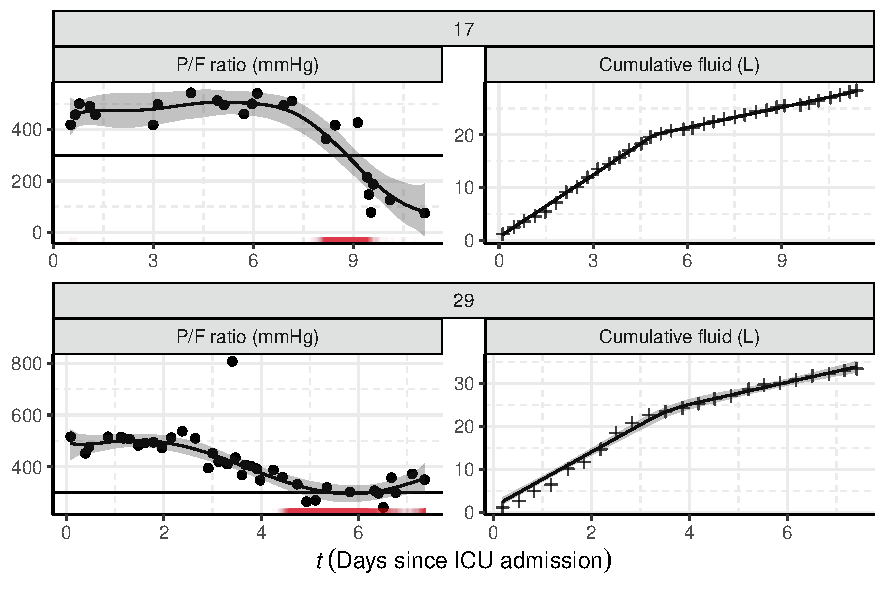
\includegraphics{../plots/mimic-example/combined-pf-fluid-fit-plot-small} 

}

\caption{The P/F ratio data ($Y_{1}$, left column); cumulative fluid data ($Y_{3}$, right column, in litres); subposterior means and 95\% credible intervals for each of the submodels (black solid lines and grey intervals); and stage one event times ($T_{i}$, red rug in left column) for individuals $i = 6, 13$, and $15$.}\label{fig:pf_fit_and_fluid_fit_plot}
\end{figure}

\hypertarget{survival-submodel-pd_2}{%
\subsection{\texorpdfstring{Survival submodel
\(\pd_{2}\)}{Survival submodel \textbackslash pd\_\{2\}}}\label{survival-submodel-pd_2}}

Individuals experience respiratory failure (\(d_{i} = 1\)) at time
\(T_{i}\), or are censored\footnote{The relationship between this model
  and the competing risks approach is discussed in Appendix
  \ref{a-comparison-with-the-competing-risk-approach}}
\((d_{i} = 2, T_{i} = C_{i})\). We assume a Weibull hazard with shape
parameter \(\gamma\) for the event times. All individuals have
\(b = 1, \ldots, B\) baseline (time invariant) covariates \(w_{i, b}\)
with
\(\boldsymbol{w}_{i} = (1, w_{i, 1}, \ldots, w_{i, B})\)(i.e.~including
an intercept term), and coefficient \(\theta \in \mathbb{R}^{B + 1}\).
The hazard is assumed to be influenced by these covariates and the rate
of increase \(\frac{\partial}{\partial t} m_{i}(t)\) in the cumulative
fluid balance. The strength of the latter relationship is captured by
\(\alpha\). Hence, the hazard is \begin{gather}
  h_{i}(T_{i}) = \gamma T_{i}^{\gamma - 1} \exp\left\{\boldsymbol{w}_{i}\theta + \alpha \frac{\partial}{\partial T_{i}} m_{i}(T_{i})\right\} \\
  \frac{\partial}{\partial T_{i}} m_{i}(T_{i}) = \eta^{b}_{1, i}\boldsymbol{1}_{\{T_{i} < \kappa_{i}\}} + \eta^{a}_{1, i}\boldsymbol{1}_{\{T_{i} \geq \kappa_{i}\}},
\end{gather}

The survival probability
\(S_{i}(T_{i}) = \exp\{-\int_{0}^{T_{i}}h_{i}(u)\text{d}u\}\) has an
analytic form, which we derive in Appendix
\ref{analytic-form-for-the-survival-probability} The likelihood for the
submodel is \begin{equation}
  \pd(T_{i}, d_{i} \mid \gamma, \boldsymbol{\theta}, \alpha, \kappa_{i}, \eta_{1, i}^{b}, \eta_{1, i}^{a}, \boldsymbol{w}_{i}) = h_{i}(T_{i})^{d_{i}} S_{i}(T_{i}), \\
\end{equation} where we suppress the dependence on the parameters on the
right hand side for brevity.

Our priors for the submodel specific parameters are \begin{equation}
\begin{gathered}
  \gamma \sim \text{Gamma}(9.05, 8.72), \, \,
  \alpha \sim \text{SkewNormal}(0, 0.5, -2), \\
  \theta_{1} \sim \text{N}(\hat{E}, 0.5^2), \, \,
  (\theta_{2}, \ldots, \theta_{B + 1}) \sim \text{SkewNormal}(0, 0.5, -1),
  \label{eqn:surv-submodel-prior-def}
\end{gathered}
\end{equation} where \(\hat{E}\) is the log of the crude event rate
(\protect\hyperlink{ref-brilleman_bayesian_2020}{Brilleman \emph{et
al.}, 2020}), and \(\boldsymbol{I}_{p}\) is the \(p \times p\) identity
matrix. Appendix \ref{p2-prior-justification} contains our justification
for these priors. We adopt the same priors as the cumulative fluid
balance submodel for \(\kappa_{i}, \eta_{1, i}^{b}\), and
\(\eta_{1, i}^{a}\).

\hypertarget{estimation-details}{%
\section{Estimation details}\label{estimation-details}}

We consider logarithmic pooling with
\(\lambda = (\frac{4}{5}, \frac{4}{5}, \frac{4}{5})\) (any smaller value
of \(\lambda\) results in a prior that is so uninformative that it
causes computational problems) and with \(\lambda = (1, 1, 1)\)
(Product-of-Experts). Because the correlation between
\(\phi_{1 \cap 2}\) and \(\phi_{2 \cap 3}\) in
\(\pd_{2}(\phi_{1 \cap 2}, \phi_{2 \cap 3})\) is important, we do not
consider linear pooling in this example. Logarithmic pooling requires
estimates of \(\pd_{1}(\phi_{1 \cap 2})\) and
\(\pd_{2}(\phi_{1 \cap 2}, \phi_{2 \cap 3})\). Because these
distributions are functions of discrete and continuous parameters
standard kernel density estimation, as suggested by
\protect\hyperlink{ref-goudie_joining_2019}{Goudie \emph{et al.}}
(\protect\hyperlink{ref-goudie_joining_2019}{2019}), is inappropriate.
Instead we fit appropriate parametric mixture distributions using Monte
Carlo samples from the priors. Samples from
\(\pd_{2}(\phi_{1 \cap 2}, \phi_{2 \cap 3})\) are obtained using the
methodology of \protect\hyperlink{ref-crowther_simulating_2013}{Crowther
and Lambert} (\protect\hyperlink{ref-crowther_simulating_2013}{2013}) as
implemented in \texttt{simsurv}
\protect\hyperlink{ref-brilleman_simsurv_2021}{Brilleman}
(\protect\hyperlink{ref-brilleman_simsurv_2021}{2021}). We will also
require an estimate of \(\pd_{2}(\phi_{1 \cap 2})\), which we obtain
using the same methodology. Further details about these estimates are
available in Appendix
\ref{estimating-submodel-prior-marginal-distributions}.

We use the parallel multi-stage sampler with
\(\pd_{\text{pool}, 1}(\phi_{1 \cap 2}) = \pd_{\text{pool}, 3}(\phi_{2 \cap 3}) \propto 1\)
and
\(\pd_{\text{pool}}(\boldsymbol{\phi}) = \pd_{\text{pool}, 2}(\phi_{1 \cap 2}, \phi_{2 \cap 3})\).
That is, in stage one we target the subposteriors
\(\pd_{1}(\phi_{1 \cap 2}, \psi_{1} \mid Y_{1})\) and
\(\pd_{3}(\phi_{2 \cap 3}, \psi_{3} \mid Y_{3})\); in stage two we
target the full melded model. The stage one subposteriors are sampled
using \texttt{Stan}, using 5 chains with 1000 warm-up iterations and
5000 post warm-up iterations. These samples are used as proposal
densities for \(\phi_{1 \cap 2}\) and \(\phi_{2 \cap 3}\) in stage two,
and we use Stan to sample \(\psi_{2}\) for every MH-within-Gibbs step,
with 9 warm-up iterations and 1 post warm-up iteration\footnote{We also
  initialise Stan at the previous value of \(\psi_{2}\), disable all
  adaptive procedures, and manually rescale the target using the
  \texttt{multiplier} syntax to ensure the default (identity) mass
  matrix is suitable. This seems to work for this example.}. We run 5
chains of 5000 samples for all stage two targets. Visual and numerical
diagnostics
(\protect\hyperlink{ref-vehtari_rank-normalization_2020}{Vehtari
\emph{et al.}, 2020}) are assessed and are available in the repository
accompanying this paper.

It is crucial for the convergence of our multi-stage sampler that the
elements of \(\phi_{1 \cap 2}\) and \(\phi_{2 \cap 3}\) are updated
individual-at-a-time. - The validity of such an updating scheme is not
immediately apparent (insofar as whether or not it has the correct
stationary distribution, nor that the cancellations of Eqs () and ()
still occur). Appendix \ref{one-at-a-time} argues that this scheme does
target the correct distribution, and that the cancellations still occur.

\hypertarget{results}{%
\section{Results}\label{results}}

To assess the impact of the melding process we compare the posterior for
\(\psi_{2}\) obtained using the chained melding approach with the
posterior obtained by fixing \(\phi_{1 \cap 2}\) and
\(\phi_{2 \cap 3}\). Specifically, we fix \(\phi_{1 \cap 2}\) to the
median value\footnote{We choose the median because the mean value of
  \(d_{i}\) is nonsensical. For each individual the samples of
  \(\{(T_{i}, d_{i})\}_{i = 1}^{N}\) sorted by \(T_{i}\), and the
  \(\lfloor \frac{N}{2}\rfloor\)\textsuperscript{th} tuple
  \((\tilde{T}_{i}, \tilde{d}_{i})\) is chosen as the median.} for each
individual under \(\pd_{1}(\phi_{1 \cap 2} \mid Y_{1})\), which we
denote \(\tilde{\phi}_{1 \cap 2}\). We fix \(\phi_{2 \cap 3}\) to the
subposterior mean of \(\pd_{3}(\phi_{2 \cap 3} \mid Y_{3})\) similarly
denoted \(\tilde{\phi}_{2 \cap 3}\). We also compare the melded
posterior to the original marginal prior \(\pd_{2}(\psi_{2})\), but we
note that this comparison is difficult to interpret, as the melding
process alters the prior for \(\psi_{2}\). Figure
\ref{fig:psi_2_comparision_plot} displays the aforementioned densities
for \((\theta_{3}, \theta_{17}, \gamma, \alpha) \subset \psi_{2}\). For
the baseline coefficients (\(\theta_{3}, \theta_{17}\)) the chained
melding posterior differs only slightly in location from the posterior
obtained using \(\tilde{\phi}_{1 \cap 2}\) and
\(\tilde{\phi}_{2 \cap 3}\), with a small increase in uncertainty. It is
interesting that the large uncertainty in \(\phi_{1 \cap 2}\) seems A
more pronounced change is visible in \(\alpha\), where the melding
process has added a notable degree of uncertainty and heavier left tail
to the posterior.

\begin{figure}

{\centering 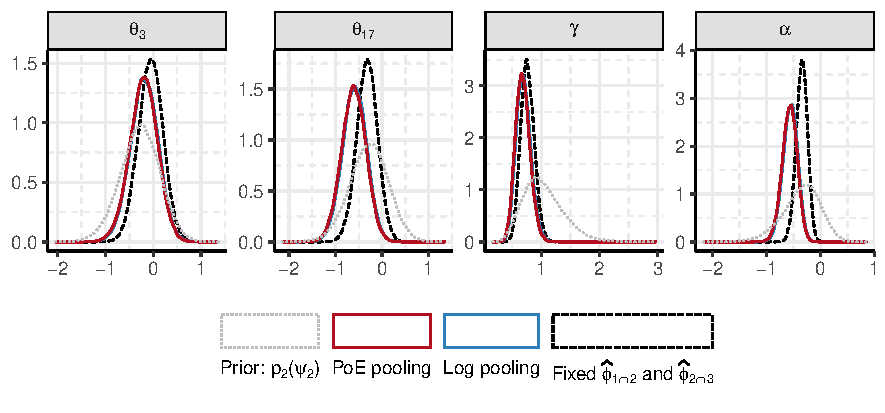
\includegraphics{../plots/mimic-example/psi-2-method-comparison-small} 

}

\caption{Density estimates for a subset of $\psi_{2}$. The original marginal prior $\pd_{2}(\psi_{2})$ is shown as the grey dotted line (note that this is not the marginal prior under the melded model). The figure also contains the subposteriors obtained from chained melding using PoE pooling (red, solid line) and logarithmic pooling (blue, solid line), as well as the posterior obtained using fixed values of $\phi_{1 \cap 2}$ and $\phi_{2 \cap 3}$ (black, dashed line).}\label{fig:psi_2_comparision_plot}
\end{figure}

To investigate which part of the melding process causes this change in
the posterior of \(\alpha\), we consider fixing only one of
\(\phi_{1 \cap 2}\) and \(\phi_{2 \cap 3}\) to their respective point
estimates. Figure \ref{fig:alpha_only_comparision_plot} displays the
same distributions for \(\alpha\) as \ref{fig:psi_2_comparision_plot},
and adds the posteriors obtained using one fixed value
(\(\tilde{\phi}_{1 \cap 2}\) or \(\tilde{\phi}_{2 \cap 3}\)) whilst
melding the other non-fixed parameter. Evident for both choices of
pooling is the importance of incorporating the uncertainty in
\(\phi_{1 \cap 2}\). This is expected given the comparatively large
uncertainty and multimodal nature of \(\phi_{1 \cap 2}\) compared to
\(\phi_{2 \cap 3}\) (see Figure \ref{fig:pf_fit_and_fluid_fit_plot}). We
suspect that it is the multimodality in
\(\pd_{1}(\phi_{1 \cap 2} \mid Y_{1})\) that produces the shift in
posterior mode of \(\phi_{1 \cap 2}\), with the width of
\(\pd_{1}(\phi_{1 \cap 2} \mid Y_{1})\) affecting the increase in
uncertainty.

\begin{figure}

{\centering 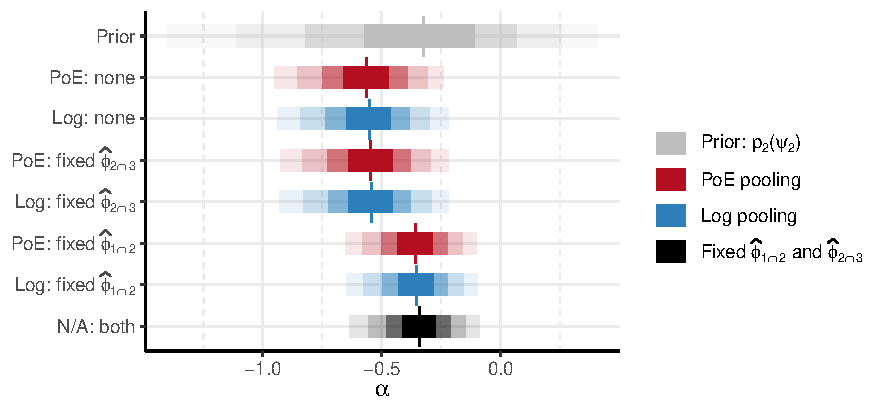
\includegraphics{../plots/mimic-example/psi-2-alpha-only-compare} 

}

\caption{Median (vertical line), 50\%, 80\%, 95\%, and 99\% credible intervals (least transparent to most transparent) for $\alpha$. The marginal prior (grey, top row) and posterior with both $\phi_{1 \cap 2}$ and $\phi_{2 \cap 3}$ fixed (black, bottom row) are as in Figure \ref{fig:psi_2_comparision_plot}. For the chained melded posteriors (red and blue, rows 2 -- 7), the tick label on the y-axis denotes the type of pooling used, and which of $\phi_{1 \cap 2}$ and $\phi_{2 \cap 3}$ are fixed.}\label{fig:alpha_only_comparision_plot}
\end{figure}

The change to the posterior distribution of \(\gamma\) in Figure
\ref{fig:psi_2_comparision_plot} appears small, however when we consider
the corresponding estimates of the survival probability, this difference
becomes much more apparent. Figure \ref{fig:kap_meier_pc_plot} displays
the average survival probability under the melded posterior (using PoE
pooling) of \(\psi_{2}\) and \(\phi_{2 \cap 3}\), and corresponding
draws of \(\phi_{1 \cap 2}\) converted into empirical survival
probabilities using the Kaplan-Meier estimator. Also shown is the
Kaplan-Meier estimate using \(\tilde{\phi}_{1 \cap 2}\), and the average
survival probability computed using the posterior of \(\psi_{2}\) with
fixed \(\tilde{\phi}_{1 \cap 2}\) and \(\tilde{\phi}_{2 \cap 3}\). The
survival curves differ markedly, with the 95\% intervals overlapping
only for small values of time. It is also interesting to see that
\(\tilde{\phi_{1 \cap 2}}\), despite being a reasonable point estimate
of \(\pd_{1}(\phi_{1 \cap 2} \mid Y_{1})\), is not very likely under the
melded posterior. Figure \ref{fig:kap_meier_pc_plot} also suggests that
the Weibull hazard is insufficiently flexible for this example, however
more complex hazards are beyond the scope of this paper\footnote{More
  complex hazards (e.g.~the default M-spline hazard in
  \protect\hyperlink{ref-brilleman_bayesian_2020}{Brilleman \emph{et
  al.}} (\protect\hyperlink{ref-brilleman_bayesian_2020}{2020})) require
  numerically integrating the hazard to obtain the survival
  probabilities. Such integrations are not trivial, particularly when
  the hazard is discontinuous, which ours is at the breakpoint.}.

\begin{figure}

{\centering 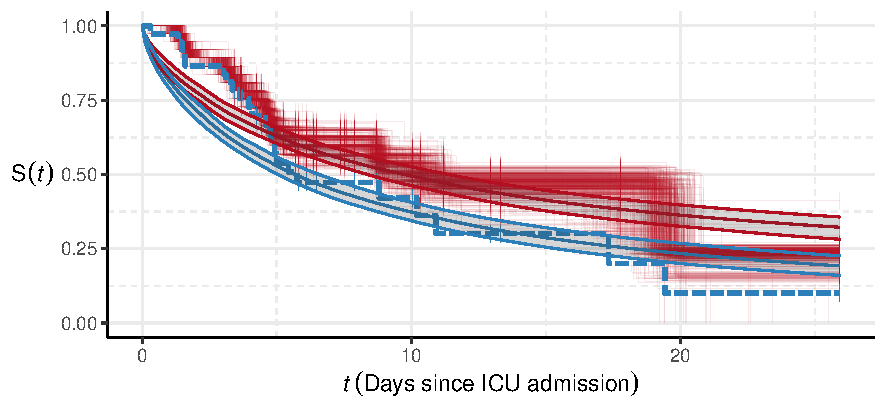
\includegraphics{../plots/mimic-example/kaplan-meier-pc} 

}

\caption{Empirical survival curves and average survival probabilities at time $t$. The black lines are draws of $\phi_{1 \cap 2}$ from the melded posterior using PoE pooling, converted into empirical survival curves via the Kaplan-Meier estimator. The red line and interval (posterior mean and 95\% credible interval) denote the model-based average survival probability obtained from the melded posterior using PoE pooling computed from the values of $\psi_{2}$ and $\phi_{2 \cap 3}$. The blue dashed line is the Kaplan-Meier estimate obtained from the subposterior median $\tilde{\phi}_{1 \cap 2}$, and the blue solid line and interval are the corresponding model based estimate obtained using $\psi_{2}$ and $\tilde{\phi}_{2 \cap 3}$.}\label{fig:kap_meier_pc_plot}
\end{figure}

\hypertarget{bibliography}{%
\section{Bibliography}\label{bibliography}}

\hypertarget{refs}{}
\begin{CSLReferences}{1}{0}
\leavevmode\hypertarget{ref-belgorodski_rriskdistributions_2017}{}%
Belgorodski, N., Greiner, M., Tolksdorf, K., et al. (2017)
{rriskDistributions}: {Fitting} distributions to given data or known
quantiles.

\leavevmode\hypertarget{ref-brilleman_simsurv_2021}{}%
Brilleman, S. (2021) Simsurv: {Simulate Survival Data}. Comprehensive R
Archive Network (CRAN).

\leavevmode\hypertarget{ref-brilleman_bayesian_2020}{}%
Brilleman, S. L., Elci, E. M., Novik, J. B., et al. (2020) Bayesian
survival analysis using the rstanarm {R} package. \emph{arXiv:2002.09633
{[}stat{]}}. Available at: \url{http://arxiv.org/abs/2002.09633}.

\leavevmode\hypertarget{ref-crowther_simulating_2013}{}%
Crowther, M. J. and Lambert, P. C. (2013) Simulating biologically
plausible complex survival data. \emph{Statistics in Medicine},
\textbf{32}, 4118--4134. DOI:
\href{https://doi.org/10.1002/sim.5823}{10.1002/sim.5823}.

\leavevmode\hypertarget{ref-gabry_visualization_2019}{}%
Gabry, J., Simpson, D., Vehtari, A., et al. (2019) Visualization in
{Bayesian} workflow. \emph{Journal of the Royal Statistical Society:
Series A (Statistics in Society)}, \textbf{182}, 389--402. DOI:
\href{https://doi.org/10.1111/rssa.12378}{10.1111/rssa.12378}.

\leavevmode\hypertarget{ref-gelman_bayesian_2020}{}%
Gelman, A., Vehtari, A., Simpson, D., et al. (2020) Bayesian workflow.
\emph{arXiv:2011.01808 {[}stat{]}}. Available at:
\url{http://arxiv.org/abs/2011.01808}.

\leavevmode\hypertarget{ref-goudie_joining_2019}{}%
Goudie, R. J. B., Presanis, A. M., Lunn, D., et al. (2019) Joining and
splitting models with {Markov} melding. \emph{Bayesian Analysis},
\textbf{14}, 81--109. DOI:
\href{https://doi.org/10.1214/18-BA1104}{10.1214/18-BA1104}.

\leavevmode\hypertarget{ref-kalbfleisch_statistical_2002}{}%
Kalbfleisch, J. D. and Prentice, R. L. (2002) \emph{The Statistical
Analysis of Failure Time Data}. 2nd ed. Wiley series in probability and
statistics. {Hoboken, N.J}: {J. Wiley}.

\leavevmode\hypertarget{ref-soetaert_rootsolve_2020}{}%
Soetaert, K., Hindmarsh, A. C., Eisenstat, S. C., et al. (2020)
{rootSolve}: {Nonlinear Root Finding}, {Equilibrium} and {Steady}-{State
Analysis} of {Ordinary Differential Equations}.

\leavevmode\hypertarget{ref-vehtari_rank-normalization_2020}{}%
Vehtari, A., Gelman, A., Simpson, D., et al. (2020) Rank-normalization,
folding, and localization: An improved \(\widehat{R}\) for assessing
convergence of {MCMC}. \emph{Bayesian Analysis}. {International Society
for Bayesian Analysis}. DOI:
\href{https://doi.org/10.1214/20-BA1221}{10.1214/20-BA1221}.

\end{CSLReferences}

\renewcommand{\thesubsection}{\Alph{subsection}}

\hypertarget{appendix}{%
\section*{Appendix}\label{appendix}}
\addcontentsline{toc}{section}{Appendix}

\hypertarget{calculating-the-cumulative-fluid-balance-from-the-raw-fluid-data}{%
\subsection{Calculating the cumulative fluid balance from the raw fluid
data}\label{calculating-the-cumulative-fluid-balance-from-the-raw-fluid-data}}

In the raw fluid data each patient has
\(\tilde{l} = 1, \ldots, \tilde{L}_{i}\) observations. Each observation
\(\tilde{x}_{i, \tilde{l}}\) is typically a small fluid administration
(e.g.~an injection of some medicine in saline solution), or a fluid
discharge (almost always urine excretion). The observations have
corresponding observation times \(\tilde{u}_{i, \tilde{l}}\), with
\(\tilde{\boldsymbol{u}}_{i} = \{\tilde{u}_{i, 1}, \ldots, \tilde{u}_{i, \tilde{L}_{i}}\}\)
and
\(\tilde{\boldsymbol{x}}_{i} = \{\tilde{x}_{i, 1}, \ldots, \tilde{x}_{i, \tilde{L}_{i}}\}\).
We code the fluid administrations/inputs as positive values, and the
excretions/outputs as negative values. Each patient has an enormous
number of raw fluid observations \((L_{i} \ll \tilde{L}_{i})\) and it is
computationally infeasible to consider them all at once. Because the
time scale of interest is typically a number of days, we aggregate the
raw fluid observations into 24-hourly changes in fluid balance. From
these 24-hourly changes we calculate the cumulative fluid balance.

Mathematically, we define an ordered integer-vector of boundary values
\begin{equation}
  \boldsymbol{b}_{i} = (\lfloor \min\{\tilde{\boldsymbol{u}}_{i}\} \rfloor,  \lfloor \min\{\tilde{\boldsymbol{u}}_{i}\} \rfloor + 1, \ldots, \lceil \max\{\tilde{\boldsymbol{u}}_{i}\} \rceil),
\end{equation} noting that \(\dim(\boldsymbol{b}_{i}) = L_{i} + 1\). The
raw fluid observations are then divided up into \(L_{i}\) subsets of
\(\{\tilde{\boldsymbol{x}}_{i}, \tilde{\boldsymbol{u}}_{i}\}\) based on
which boundary values the observation falls in between: \begin{equation}
  B_{i, l} = \left\{
    \{\tilde{\boldsymbol{x}}_{i}, \tilde{\boldsymbol{u}}_{i}\}
    \mid
    b_{i, l} \leq \tilde{\boldsymbol{u}}_{i} < b_{i, l + 1}
  \right\},
\end{equation} for \(l = 1, \ldots, L_{i}\). Denote
\(N^{B}_{i, l} = \lvert B_{i, l} \rvert \mathop{/} 2\) (dividing by two
as \(B_{i, l}\) contains both the observation and the observation time).
The \(l\)\textsuperscript{th} 24-hourly fluid change \(\Delta_{i, l}\)
and corresponding observation time \(u_{i, l}\) can then be computed as
\begin{equation}
  \Delta_{i, l} = \sum_{s = 1}^{N^{B}_{i, l}} \tilde{x}_{i, s}, \,\, \text{s.t.} \,\, \tilde{x}_{i, s} \in B_{i, l}, \qquad
  u_{i, l} = \frac{1}{N^{B}_{i, l}} \sum_{s = 1}^{N^{B}_{i, l}} \tilde{u}_{i, s}, \,\, \text{s.t.} \,\, \tilde{u}_{i, s} \in B_{i, l}.
\end{equation} Finally, the 24-hourly cumulative fluid balance data are
computed by \(x_{i, l} = \sum_{s = 1}^{l} \Delta_{i, s}\), and we assume
they too are observed at \(u_{i, l}\).

\hypertarget{priors-and-justification-for-the-fluid-submodel}{%
\subsection{Priors and justification for the fluid
submodel}\label{priors-and-justification-for-the-fluid-submodel}}

We assume a weakly informative prior for the error term \begin{equation}
  \epsilon_{i, l} \sim \text{N}(0, \sigma^{2}_{x}),  \,\, \sigma_{x} \sim \text{N}_{+}(0, 5^2).
\end{equation}

The parameters for the gamma prior for \(\eta^{b}_{1, i}\) and
\(\eta^{a}_{1, i}\) are obtained by assuming that the 2.5-, 50-, and
97.5- percentiles are at 0.5, 5, and 20
(\protect\hyperlink{ref-belgorodski_rriskdistributions_2017}{Belgorodski
\emph{et al.}, 2017}). A slope of \(0.5\) (i.e.~the change in cumulative
fluid balance per day) is unlikely but possible due to missing data; a
slope of \(20\) is also unlikely but possible as extremely unwell
patients can have very high respiratory rates and thus require large
fluid inputs. Thus \begin{equation}
  \eta^{b}_{1, i} \sim \text{Gamma}(1.53, 0.24), \,\, \eta^{a}_{1, i} \sim \text{Gamma}(1.53, 0.24).
\end{equation}

The prior for the breakpoint \(\kappa_{i}\) is derived as follows.
Define \(u_{i, (1)} = \min(\boldsymbol{u}_{i})\) and
\(u_{i, (n)} = \max(\boldsymbol{u}_{i})\), with
\(r_{i} = u_{i, (n)} - u_{i, (1)}\). We reparameterise the breakpoint by
noting that \(\kappa_{i} = \kappa^{\text{raw}}_{i}r_{i} + u_{i, (1)}\),
where \(\kappa^{\text{raw}} \in [0, 1]\). We then set
\(\kappa^{\text{raw}}_{i} \sim \text{Beta}(5, 5)\) to regularise the
breakpoint towards the middle of each individual's stay in ICU. This is
crucial to ensure the submodel is identifiable when there is little
evidence of a breakpoint in the data. Note that this results in the
following analytic expression for \(\pd_{2}(\phi_{2 \cap 3})\)
\begin{equation}
  \pd_{3}(\phi_{2 \cap 3}) = \prod_{i = 1}^{N} \pd(\eta^{b}_{1, i}) \pd(\eta^{a}_{1, i}) \pd(\kappa_{i}), \,\, \text{with} \,\,\,
  \pd(\kappa_{i}) = \pd_{\kappa^{\text{raw}}_{i}}\left(\frac{\kappa_{i} - u_{i, (1)}}{r_{i}}\right) \frac{1}{r_{i}}
\end{equation} by the change of variables formula.

Specifying a prior for \(\eta_{0, i}\), the cumulative fluid balance at
\(\kappa_{i}\), is difficult because it depends on the length of stay.
Instead, we reparameterise so that \(\eta_{0, i}\) is a function of the
y-intercept \(\eta_{0, i}^{\text{raw}}\). \begin{equation}
  \eta_{0, i} =
    (\eta_{0, i}^{\text{raw}} + \eta^{b}_{1, i} \kappa_{i}) \boldsymbol{1}_{\{0 < \kappa_{i}\}} +
    (\eta_{0, i}^{\text{raw}} + \eta^{a}_{1, i} \kappa_{i}) \boldsymbol{1}_{\{0 \geq \kappa_{i}\}}
\end{equation} We place a \(\text{LogNormal}(1.61, 0.47^2)\) prior on
\(\eta_{0, i}^{\text{raw}}\). These values are obtained assuming that, a
priori, the \(2.5\%, 50\%\), and \(99\%\) percentiles of
\(\eta_{0, i}^{\text{raw}}\) are \(0.5, 5\), and \(15\) respectively
(\protect\hyperlink{ref-belgorodski_rriskdistributions_2017}{Belgorodski
\emph{et al.}, 2017}). This is a broad prior that reflects the numerous
possible admission routes into the ICU. We expect those admitted from
the wards to have little pre-admission fluid data. Those admitted from
the operating theatre occasionally have their in-theatre fluid input
recorded after admission into the ICU, with no easy way to distinguish
these records in the data.

\hypertarget{a-comparison-with-the-competing-risk-approach}{%
\subsection{A comparison with the competing risk
approach}\label{a-comparison-with-the-competing-risk-approach}}

An alternative approach is to consider a competing risks model for
\(\pd_{2}\), where each individual experiences either the respiratory
failure event or the competing, non-independent event of death or
discharge (see Chapter 8 of
\protect\hyperlink{ref-kalbfleisch_statistical_2002}{Kalbfleisch and
Prentice, 2002} for an introduction). However, issues arise due to the
difference in supports between \(\pd_{1}(\phi_{1 \cap 2})\) and
\(\pd_{2}(\phi_{1 \cap 2})\); aligning the supports requires
conditioning on \(C_{i}\) (the length of stay) in \(\pd_{2}\).
Conditional on \(C_{i}\), the death or discharge event can only happen
at a known, fixed time, which violates the competing risk assumption
(that each event can occur at any moment in time the individual is
exposed to both risks). In light of this, we feel that it is more
correct to consider the time of death or discharge as a censoring time.
Standard survival analyses arguments show us that these approaches are
equivalent subject to certain assumptions. However, one key these
arguments make is that the survival times and indicators
\((T_{i}, d_{i})\) must be known/fixed quantities. This assumption is
not valid in our example, and below we show why this invalidates the
usual equivalence between the competing risk and censoring approaches.

Suppose that each individual \(i\) experiences one of \(d_{i} = 1, 2\)
competing risks. We observe \(\{T_{i}, d_{i}\}\), where \(d_{i} = 1\)
indicates that individual \(i\) experienced respiratory failure at time
\(T_{i}\). If \(d_{i} = 2\) then individual \(i\) expired or was
discharged at time \(T_{i}\), noting that this event must occur at time
\(C_{i}\). Each cause-specific hazard has parameters \(\theta_{d_{i}}\)
and we denote the hazard
\(h_{i, d_{i}}(t \mid \theta_{d_{i}}, \boldsymbol{w}_{i})\). Denote
\(\boldsymbol{\theta} = (\theta_{1}, \theta_{2})\) and assume only one
such event can occur at a time so that \begin{gather}
  h_{i}(T_{i} \mid \boldsymbol{\theta}, \boldsymbol{w}_{i}) = \sum_{d_{i} \in \{1, 2\}} h_{i, d_{i}}(T_{i} \mid \theta_{d_{i}}, \boldsymbol{w}_{i}), \\
  \begin{aligned}
  H_{i}(T_{i} \mid \boldsymbol{\theta}, \boldsymbol{w}_{i})
    &= \int_{0}^{T_{i}} \sum_{d_{i} \in \{1, 2\}} h_{i, d_{i}}(u \mid \theta_{d_{i}}, \boldsymbol{w}_{i}) \text{d}u \\
    &= \sum_{d_{i} \in \{1, 2\}} \int_{0}^{T_{i}} h_{i, d_{i}}(u \mid \theta_{d_{i}}, \boldsymbol{w}_{i}) \text{d}u \\
    &= \sum_{d_{i} \in \{1, 2\}} H_{i, d_{i}}(T_{i} \mid \theta_{d_{i}}, \boldsymbol{w}_{i}),
  \end{aligned} \\
  S_{i}(T_{i} \mid \boldsymbol{\theta}, \boldsymbol{w}_{i})
    = \exp\left\{-H_{i}(T_{i} \mid \boldsymbol{\theta}, \boldsymbol{w}_{i})\right\}
    = \exp\left\{-\sum_{d_{i} \in \{1, 2\}} H_{i, d_{i}}(T_{i} \mid \theta_{d_{i}}, \boldsymbol{w}_{i})\right\}.
\end{gather} As per Equation (8.8) in
\protect\hyperlink{ref-kalbfleisch_statistical_2002}{Kalbfleisch and
Prentice} (\protect\hyperlink{ref-kalbfleisch_statistical_2002}{2002})
the likelihood function for a specific individual is \begin{align*}
  \pd(T_{i}, d_{i} \mid \boldsymbol{\theta}, \boldsymbol{w}_{i})
    &= h_{i, d_{i}}(T_{i} \mid \theta_{d_{i}}, \boldsymbol{w}_{i}) S_{i}(T_{i} \mid \boldsymbol{\theta}, \boldsymbol{w}_{i}) \\
    &= h_{i, d_{i}}(T_{i} \mid \theta_{d_{i}}, \boldsymbol{w}_{i}) \exp\left\{-\sum_{d_{i} \in \{1, 2\}} H_{i, d_{i}}(T_{i} \mid \theta_{d_{i}}, \boldsymbol{w}_{i})\right\}.
\end{align*}

It is now necessary to assume

\begin{itemize}
\tightlist
\item
  that there are no shared elements in \(\theta_{1}\) and \(\theta_{2}\)
  and they are a priori independent,
\item
  that \(\theta_{2}\) is not of interest, i.e.~we wish to
  integrate/marginalise \(\theta_{2}\) out of the likelihood.
\end{itemize}

The model (given covariates \(\boldsymbol{w}_{i}\)) is

\begin{equation}
  \pd(T_{i}, d_{i}, \boldsymbol{\theta} \mid \boldsymbol{w}_{i}) =
    \pd(T_{i}, d_{i} \mid \boldsymbol{\theta}, \boldsymbol{w}_{i})\pd(\boldsymbol{\theta}).
\end{equation}

We are interested in the following marginal

\begin{equation}
  \pd(T_{i}, d_{i}, \theta_{1} \mid \boldsymbol{w}_{i})
  = \int \pd(T_{i}, d_{i}, \boldsymbol{\theta} \mid \boldsymbol{w}_{i}) \text{d}\theta_{2}
  = \int h_{i, d_{i}}(T_{i} \mid \theta_{d_{i}}, \boldsymbol{w}_{i}) S_{i}(T_{i} \mid \boldsymbol{\theta}, \boldsymbol{w}_{i}) \pd(\theta_{1}) \pd(\theta_{2}) \text{d}\theta_{2}.
\end{equation} If \(d_{i} = 1\) \begin{equation}
  \pd(T_{i}, d_{i}, \theta_{1} \mid \boldsymbol{w}_{i})
  = h_{i, 1}(T_{i} \mid \theta_{1}, \boldsymbol{w}_{i}) S_{i, 1}(T_{i} \mid \theta_{1}, \boldsymbol{w}_{i}) \pd(\theta_{1}) \int S_{i, 2}(T_{i} \mid \theta_{2}, \boldsymbol{w}_{i}) \pd(\theta_{2}) \text{d} \theta_{2},
  \label{eqn:competing-risks-deriv-one}
\end{equation} and if \(d_{i} = 2\) \begin{equation}
  \pd(T_{i}, d_{i}, \theta_{1} \mid \boldsymbol{w}_{i})
  = S_{i, 1}(T_{i} \mid \theta_{1}, \boldsymbol{w}_{i}) \pd(\theta_{1}) \int h_{i, 2}(T_{i} \mid \theta_{2}, \boldsymbol{w}_{i}) S_{i, 2}(T_{i} \mid \theta_{2}, \boldsymbol{w}_{i}) \pd(\theta_{2}) \text{d} \theta_{2}.
  \label{eqn:competing-risks-deriv-two}
\end{equation} Standard survival analyses consider \(T_{i}\) as data.
Under this assumption the integrals in
\eqref{eqn:competing-risks-deriv-one} and
\eqref{eqn:competing-risks-deriv-two} are constants that do not depend
on the parameters of interest, and can be ignored when maximising the
likelihood for \(\theta_{1}\). The remaining components of
\eqref{eqn:competing-risks-deriv-one} and
\eqref{eqn:competing-risks-deriv-two} comprise the likelihood that would
be obtained by considering all non \(d_{i} = 1\) events as censored.
However, in our case \(T_{i}\) is a parameter, and hence the integrals
are non-ignorable functions of \(T_{i}\). This implies that the
censoring model and the competing risks model are not equivalent, which
we see in practice when comparing the posterior distributions for
\(\theta_{1}\) under both models.

\hypertarget{analytic-form-for-the-survival-probability}{%
\subsection{Analytic form for the survival
probability}\label{analytic-form-for-the-survival-probability}}

The hazard at arbitrary time \(t\) is

\begin{gather*}
  h_{i}(t) = \gamma t^{\gamma - 1} \exp\left\{\boldsymbol{x}_{i}\theta + \alpha \frac{\partial}{\partial t} m_{i}(t)\right\} \\
  m_{i}(t) = \eta_{0, i} + \eta^{b}_{1, i}(t - k_{i})\boldsymbol{1}_{\{t < k_{i}\}} + \eta^{a}_{1, i}(t - k_{i})\boldsymbol{1}_{\{t \geq k_{i}\}} \\
  \frac{\partial}{\partial t} m_{i}(t) = \eta^{b}_{1, i}\boldsymbol{1}_{\{t < k_{i}\}} + \eta^{a}_{1, i}\boldsymbol{1}_{\{t \geq k_{i}\}}.
\end{gather*}

Then, for \(t > k_{i}\), the cumulative hazard is

\begin{align*}
  \int_{0}^{t} h_{i}(u) \text{d}u
  &= \int_{0}^{t}
    \gamma u^{\gamma - 1}
    \exp\left\{
      \boldsymbol{x}_{i}\theta +
      \alpha \eta^{b}_{1, i}\boldsymbol{1}_{\{u < k_{i}\}} +
      \alpha \eta^{a}_{1, i}\boldsymbol{1}_{\{u \geq k_{i}\}}
    \right\}
    \text{d}u \\
  &= \gamma \exp\{\boldsymbol{x}_{i}\theta\}
    \int_{0}^{t}
      u^{\gamma - 1}
      \exp\left\{
        \alpha \eta^{b}_{1, i}\boldsymbol{1}_{\{u < k_{i}\}} +
        \alpha \eta^{a}_{1, i}\boldsymbol{1}_{\{u \geq k_{i}\}}
      \right\}
    \text{d}u \\
  &= \gamma \exp\{\boldsymbol{x}_{i}\theta\}
    \left[
      \int_{0}^{k_{i}}
        u^{\gamma - 1}
        \exp\left\{
          \alpha \eta^{b}_{1, i}
        \right\}
      \text{d}u
      +
      \int_{k_{i}}^{t}
        u^{\gamma - 1}
        \exp\left\{
          \alpha \eta^{a}_{1, i}
        \right\}
      \text{d}u
    \right] \\
  &= \exp\{\boldsymbol{x}_{i}\theta\}
    \left[
      \exp\left\{
        \alpha \eta^{b}_{1, i}
      \right\}
      k_{i}^{\gamma}
      +
      \exp\left\{
        \alpha \eta^{a}_{1, i}
      \right\}
      (t^{\gamma} - k_{i}^{\gamma})
    \right]
\end{align*}

and for \(t < k_{i}\)

\begin{align*}
  \int_{0}^{t} h_{i}(u) \text{d}u
  &= \gamma \exp\{\boldsymbol{x}_{i}\theta\}
    \left[
      \int_{0}^{t}
        u^{\gamma - 1}
        \exp\left\{
          \alpha \eta^{b}_{1, i}
        \right\}
      \text{d}u
    \right] \\
  &= \exp\{\boldsymbol{x}_{i}\theta\}
    \left[
      \exp\left\{
        \alpha \eta^{b}_{1, i}
      \right\}
      t_{i}^{\gamma}
    \right] \\
  &= t_{i}^{\gamma} \exp\{\boldsymbol{x}_{i}\theta + \alpha \eta^{b}_{1, i}\}.
\end{align*} The survival probabilities are defined with appropriately
for \(t > k_{i}\) and \(t < k_{i}\) as
\(S_{i}(t) = \exp\{-\int_{0}^{t} h_{i}(u) \text{d}u\}\).

\hypertarget{p2-prior-justification}{%
\subsection{Survival submodel prior
justification}\label{p2-prior-justification}}

Our prior for \((\gamma, \alpha, \boldsymbol{\theta})\) must result in a
plausible distribution for \(\pd_{2, i}(T_{i} \mid d_{i} = 1)\), and a
reasonable balance between \(d_{i} = 1\) and \(d_{i} = 0\) events. The
primary concern is unintentionally specifying a prior for which the bulk
of \(\pd_{2, i}(T_{i} \mid d_{i} = 1)\) is very close to zero. In
addition, certain extreme configurations of
\((\gamma, \alpha, \boldsymbol{\theta})\) cause issues for the
methodology of \protect\hyperlink{ref-crowther_simulating_2013}{Crowther
and Lambert} (\protect\hyperlink{ref-crowther_simulating_2013}{2013}),
particularly the numerical root finding and numerical integration steps.
We would like to rule out such extreme configurations a priori. Ideally
we would encode this information a joint prior for
\((\gamma, \alpha, \boldsymbol{\theta})\), but specifying the
appropriate correlation structure for these parameters is prohibitively
challenging. Instead we focus on specifying appropriate marginals for
each of \(\gamma, \alpha\), and \(\boldsymbol{\theta}\), and create
visual prior predictive checks
(\protect\hyperlink{ref-gabry_visualization_2019}{Gabry \emph{et al.},
2019}; \protect\hyperlink{ref-gelman_bayesian_2020}{Gelman \emph{et
al.}, 2020}) to ensure the induced prior for \((T_{i}, d_{i})\) is
acceptable.

Before justifying our chosen marginal priors is, we note that the
\(\exp\{\boldsymbol{x}_{i}\theta + \alpha \frac{\partial}{\partial T_{i}} m_{i}(T_{i})\}\)
term implies that the priors for \(\theta\) and \(\alpha\) are on the
log-scale. Hence the magnitude of these parameters must be small,
otherwise all event times would be very near zero or at infinity. The
non-symmetric effect of the transformation from the log scale also
implies that symmetric priors are not obviously sensible. From these
observations we deduce that \(\theta\) and \(\alpha\) must not be too
large in magnitude, however if they are negative then they can be
slightly larger. Hence, we specify the skew-normal priors detailed in
Equation \eqref{eqn:surv-submodel-prior-def}, noting that the skewness
parameter for \(\alpha\) is smaller, because
\(\frac{\partial}{\partial T_{i}} m_{i}(T_{i})\) is strictly positive
and typically between 0.5 and 20, whilst \(\boldsymbol{w}_{i}\) is
standardised to be approximately standard normal. Lastly, if \(\gamma\)
is too far away from \(1\) (in either direction), then the event times
are very small either because the hazard increases rapidly
(\(\gamma \gg 1\)), or because almost all of the cumulative hazard is in
the neighbourhood of 0 (\(\gamma \ll 1\)). We specify a gamma
distribution for \(\gamma\) with the \(1\)\textsuperscript{th}-,
\(50\)\textsuperscript{th}-, and \(99\)\textsuperscript{th}-percentiles
of \(\pd_{2}(\gamma)\) are at \(0.2, 1\), and \(2\), allowing for a wide
range of hazard shapes, but removing many of the extremes.

\hypertarget{estimating-submodel-prior-marginal-distributions}{%
\subsection{Estimating submodel prior marginal
distributions}\label{estimating-submodel-prior-marginal-distributions}}

\hypertarget{pf-submodel}{%
\subsubsection{P/F submodel}\label{pf-submodel}}

We approximate \(\pd_{1}(\phi_{1 \cap 2})\) using a mixture of discrete
and continuous distributions, with a discrete spike at \(C_{i}\) for the
censored events and a beta distribution for the (rescaled) event times.
Monte Carlo samples of \(T_{i}\) and \(d_{i}\) are obtained from
\(\pd_{1, i}(T_{i}, d_{i})\) by drawing \(\beta_{0, i}\) and
\(\boldsymbol{\zeta}_{i}\) from their respective prior distributions and
then solving \eqref{eqn:event_time_model_def}. Denoting the estimated
mixture weight \(\widehat{\pi}_{i} \in [0, 1]\), the density estimate is
\begin{equation}
  \widehat{\pd}_{1, i}(T_{i}, d_{i}) =
    \widehat{\pi}_{i} \, \text{Beta}\left(\frac{T_{i}}{C_{i}}; \widehat{a}, \widehat{b}\right) \frac{1}{C_{i}} \boldsymbol{1}_{\{d_{i} = 1\}} +
    (1 - \widehat{\pi}_{i}) \boldsymbol{1}_{\{d_{i} = 2, T_{i} = C_{i}\}}
  \label{eqn:pf-event-time-prior-dist}
\end{equation} where \(\widehat{\pi}_{i}, \widehat{a}_{i}\) and
\(\widehat{b}_{i}\) are maximum likelihood estimates obtained using the
prior samples. Examples of \(\widehat{\pd}_{1, i}(T_{i}, d_{i})\) for a
subset of individuals are displayed in Figure \ref{fig:pf_prior_fit}.

\begin{figure}

{\centering 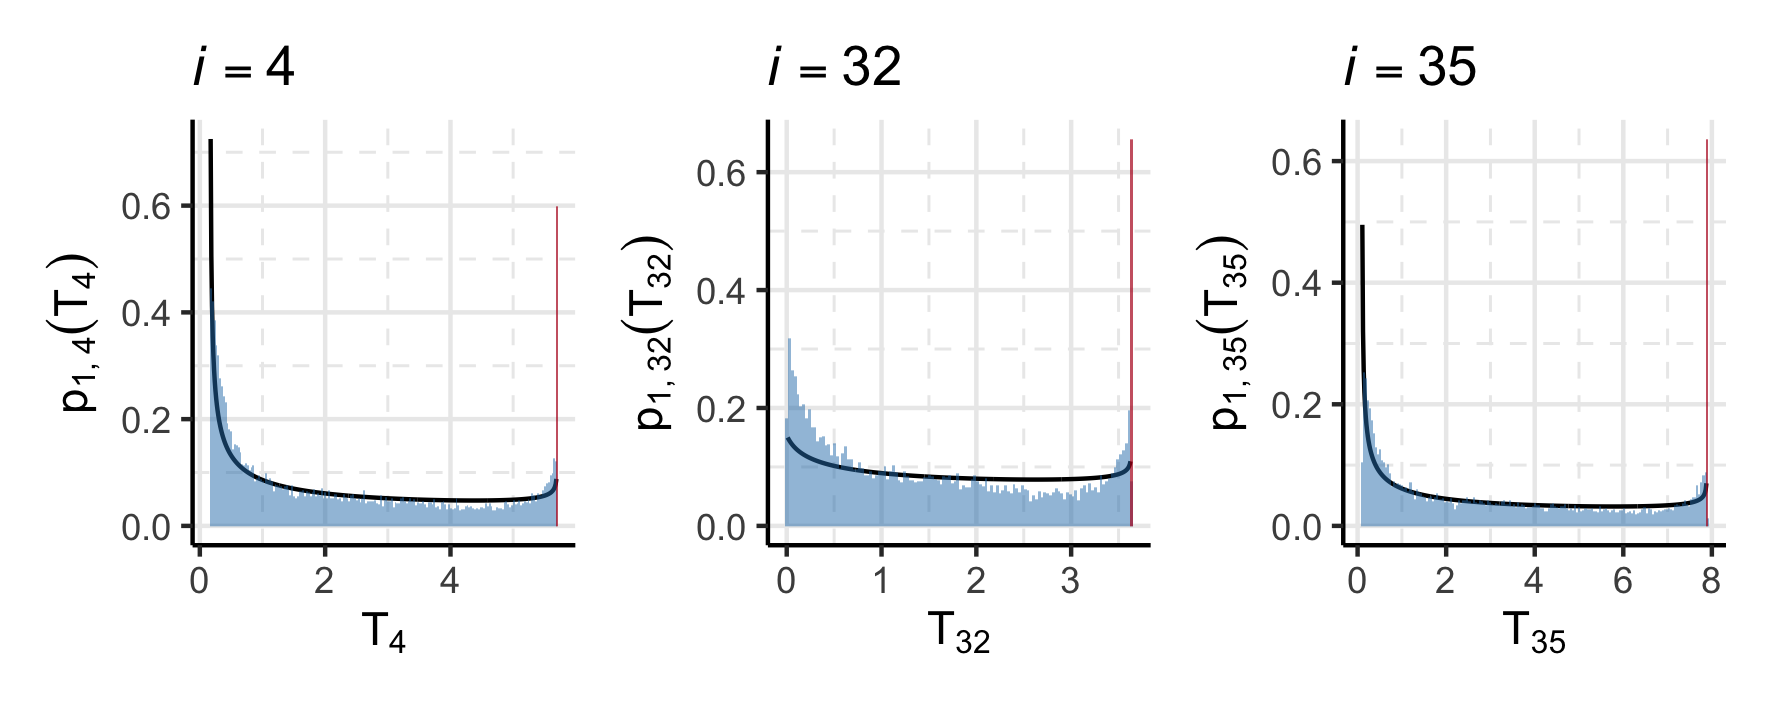
\includegraphics{../plots/mimic-example/pf-prior-plot-small} 

}

\caption{Fitted distribution (curve) and Monte Carlo samples drawn from $\pd_{1}(\phi_{1 \cap 2})$ (histogram) for a subset of the individuals in the cohort. The height of the atom at $C_{i}$ (red bar and point) has been set to $1 - \widehat{\pi}_{i}$}\label{fig:pf_prior_fit}
\end{figure}

\hypertarget{survival-submodel}{%
\subsubsection{Survival submodel}\label{survival-submodel}}

Our estimate of \(\pd_{2}(\phi_{1 \cap 2}, \phi_{2 \cap 3})\) relies on
the fact that
\(\pd_{2}(\phi_{1 \cap 2}, \phi_{2 \cap 3}) = \prod_{i = 1}^{N}\pd_{2, i}(T_{i}, d_{i}, \kappa_{i}, \eta^{b}_{1, i}, \eta^{a}_{1, i})\).
As such we estimate
\(\pd_{2, i}(T_{i}, d_{i}, \kappa_{i}, \eta^{b}_{1, i}, \eta^{a}_{1, i})\)
for each individual and take the product of these estimates. Drawing
samples from
\(\pd_{2, i}(T_{i}, d_{i}, \kappa_{i}, \eta^{b}_{1, i}, \eta^{a}_{1, i})\)
is challenging: we use the approach proposed by
\protect\hyperlink{ref-crowther_simulating_2013}{Crowther and Lambert}
(\protect\hyperlink{ref-crowther_simulating_2013}{2013}) as implemented
in \protect\hyperlink{ref-brilleman_simsurv_2021}{Brilleman}
(\protect\hyperlink{ref-brilleman_simsurv_2021}{2021}). Inspecting the
samples reveals correlation between \((T_{i}, d_{i})\) and
\((\kappa_{i}, \eta^{b}_{1, i}, \eta^{a}_{1, i})\) that we would like to
capture in our estimate. To do so, we fit a mixture of multivariate
normal distributions to transformations of the continuous parameters
with support on \(\mathbb{R}\), \begin{equation}
  \tilde{T}_{i} = \text{Logit}\left(\frac{T_{i}}{C_{i}}\right), \quad
  \tilde{\kappa}_{i} = \text{Logit}\left(\frac{\kappa_{i} - u_{i, (1)}}{u_{i, (n)} - u_{i, (1)}}\right), \quad
  \tilde{\eta}^{b}_{1, i} = \log(\eta^{b}_{1, i}), \quad
  \tilde{\eta}^{a}_{1, i} = \log(\eta^{a}_{1, i}).
\end{equation} The resulting density estimate, with estimated mixture
weight \(\widehat{\theta}_{i} \in [0, 1]\), is \begin{align*}
  \widehat{\pd}_{2}(T_{i}, d_{i}, \kappa_{i}, \eta^{b}_{1, i}, \eta^{a}_{1, i}) =
    \Big[&(\widehat{\theta}_{i})
    \text{N}\left(\left[\tilde{T}_{i}, \tilde{\kappa}_{i}, \tilde{\eta}^{b}_{1, i}, \tilde{\eta}^{a}_{1, i} \right]^{\top}; \widehat{\mu}_{1, i}, \widehat{\Sigma}_{1, i} \right) \
    \boldsymbol{1}_{\{d_{i} = 1\}}
    + \\
    &(1 - \widehat{\theta}_{i})
    \text{N}\left(\left[\tilde{\kappa}_{i}, \tilde{\eta}^{b}_{1, i}, \tilde{\eta}^{a}_{1, i} \right]^{\top}; \widehat{\mu}_{0, i}, \widehat{\Sigma}_{0, i} \right) \
    \boldsymbol{1}_{\{d_{i} = 0, T_{i} = C_{i}\}} \Big]
    J_{i},
\end{align*} where
\(\widehat{\theta}_{i}, \widehat{\mu}_{1, i}, \widehat{\Sigma}_{1, i}, \widehat{\mu}_{0, i}\),
and \(\widehat{\Sigma}_{0, i}\) are maximum likelihood estimates, and
the Jacobian correction \(J_{i}\) is \begin{equation}
  J_{i} = \left[
    \left(
      \frac{1}{C_{i} - T_{i}} +
      \frac{1}{T_{i}}
    \right)^{d_{i}}
    \left(
      \frac{1}{u_{i, (n)} - \kappa_{i}} +
      \frac{1}{\kappa_{i} - u_{i, (1)}}
    \right)
    \left(
      \frac{1}{\eta^{b}_{1, i}}
    \right)
    \left(
      \frac{1}{\eta^{a}_{1, i}}
    \right)
  \right].
\end{equation}

We asses the fit of this estimate by drawing samples from
\(\widehat{\pd}_{2, i}(\phi_{1 \cap 2}, \phi_{2 \cap 3})\) and comparing
them to the Monte Carlo samples drawn using \texttt{simsurv}. Our visual
assessment is displayed in Figure \ref{fig:surv_prior_plot_fit} for
individual \(i = 19\). The normal approximation seems to fit the samples
well, with the shape of \(\pd_{2, i}(T_{i} \mid d_{i} = 1)\) closely
matching that of the Monte Carlo samples, and with a similar mix of
\(d_{i} = 0\) and \(d_{i} = 1\) samples.

We also require an estimate of \(\pd_{2}(\phi_{1 \cap 2})\) for
experiments discussed in Section \ref{results}. This is obtained using
the samples generated under the survival submodel prior and the
methodology of Section \ref{pf-submodel}. The raw samples and fit are
displayed in Figure \ref{fig:surv_prior_phi_12_marginal_plot_fit}.

\begin{figure}

{\centering 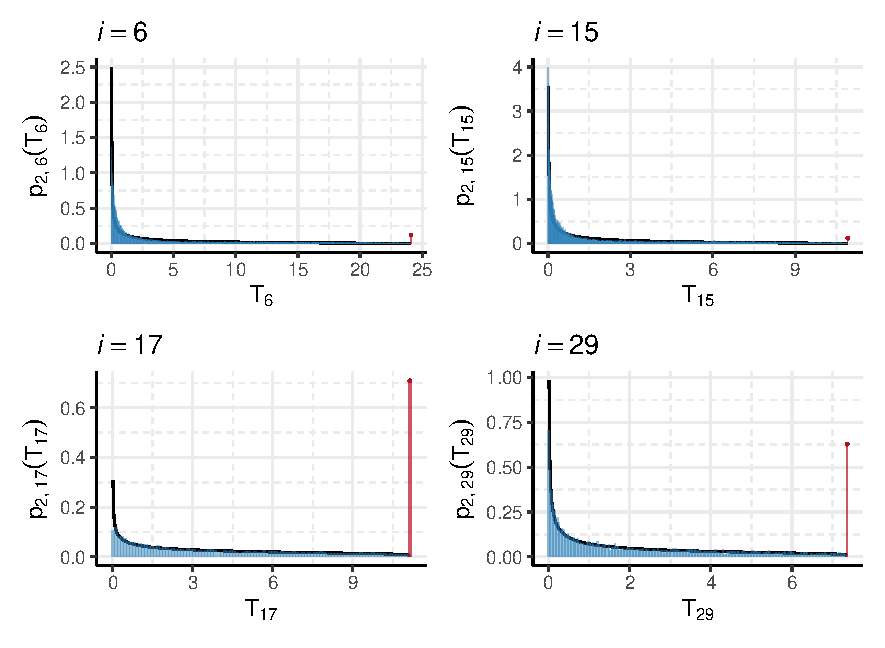
\includegraphics{../plots/mimic-example/submodel-2-phi-12-marginal-fit-plot-small} 

}

\caption{Fitted distribution (curve) and Monte Carlo samples drawn from $\pd_{2}(\phi_{1 \cap 2})$ (histogram) for a subset of the individuals in the cohort. The height of the atom at $C_{i}$ (red bar and point) has been set to $1 - \widehat{\theta}_{i}$}\label{fig:surv_prior_phi_12_marginal_plot_fit}
\end{figure}

\begin{figure}

{\centering 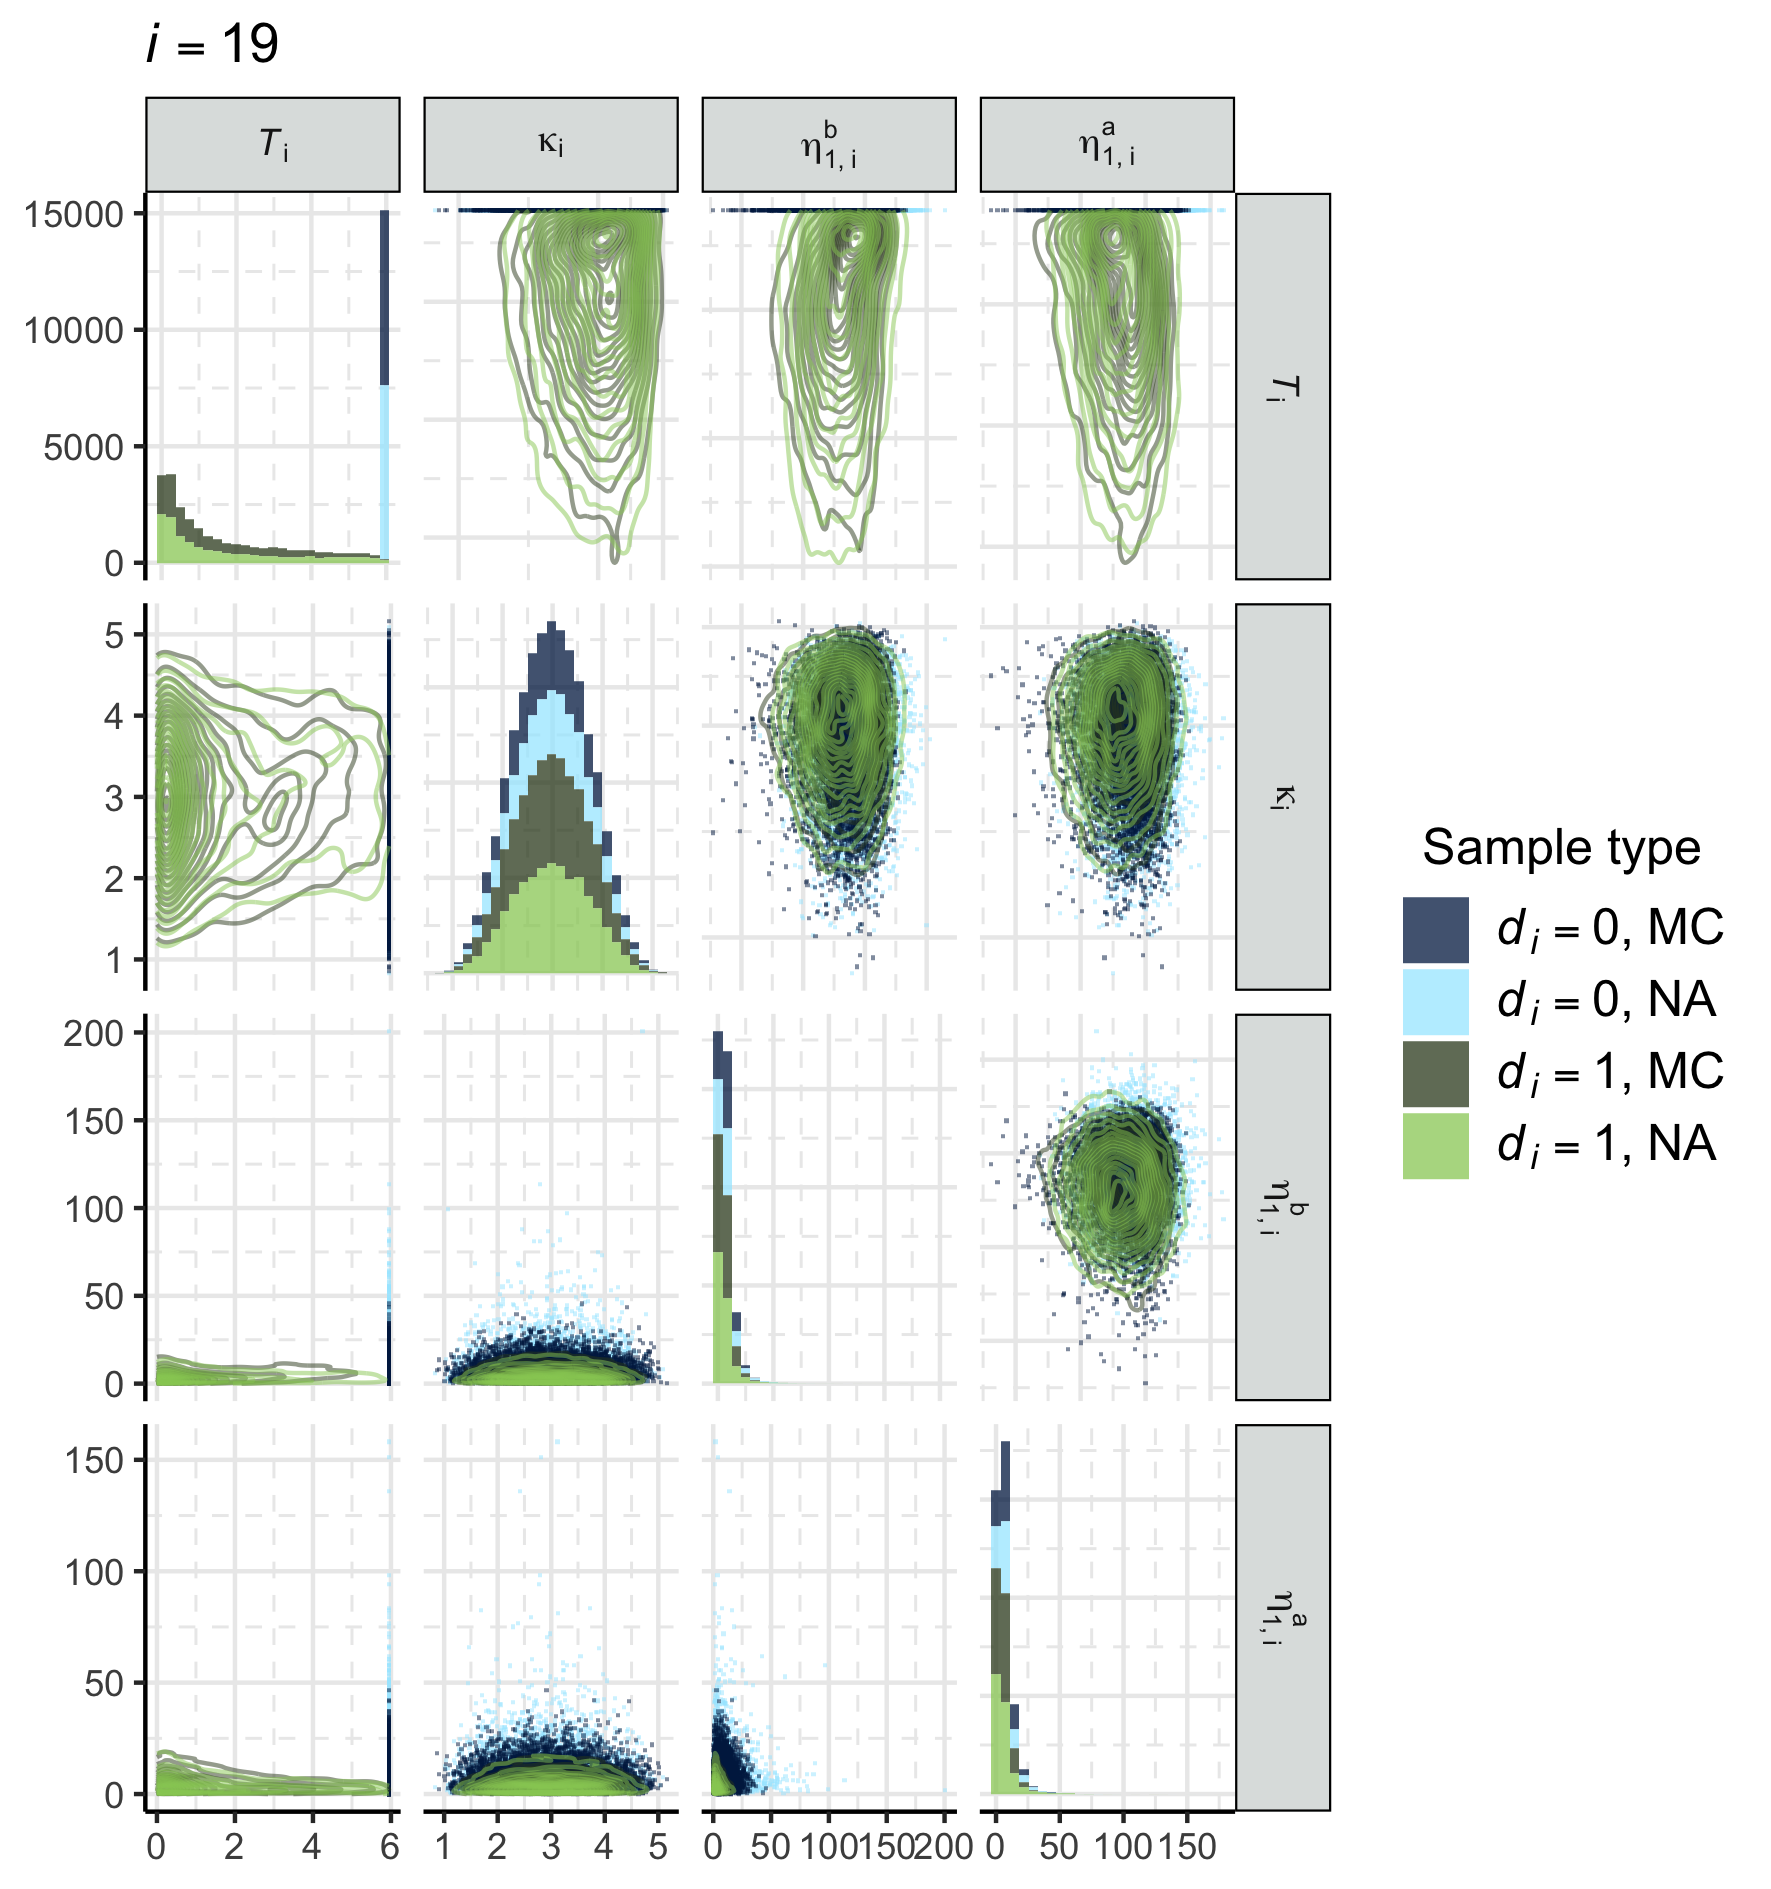
\includegraphics{../plots/mimic-example/p3-prior-pairs/pairs-19} 

}

\caption{Monte Carlo (MC) samples from $\pd_{2, i}(\phi_{1 \cap 2}, \phi_{2 \cap 3})$ obtained using \texttt{simsurv} and samples from the fitted normal approximation (NA) for $i = 19$. The panels on the off diagonal elements contain a 2D kernel density estimate for $d_{i} = 1$ and the samples for $d_{i} = 0$. Diagonal and lower-triangular panels are on their original scales, whilst the upper-triangular panels are on the log scale.}\label{fig:surv_prior_plot_fit}
\end{figure}

\hypertarget{cohort-selection-criteria}{%
\subsection{Cohort selection criteria}\label{cohort-selection-criteria}}

This appendix details the cohort selection criteria and our rationale
for them. In the text we speak of the \(i\)\textsuperscript{th}
individual. This is because in our final data set (the data that results
from applying the following criteria) we are dealing with unique
individuals, however some individuals in MIMIC have multiple ICU stays.
In this appendix \(i\) represents a single stay in ICU.

\begin{enumerate}
\def\labelenumi{\arabic{enumi}.}
\tightlist
\item
  Each ICU stay must have at least 12 PF observations (\(z_{i, j}\) with
  \(J_{i} \geq 12\)), with the first 6 being greater than 350.

  \begin{itemize}
  \tightlist
  \item
    This is to ensure we have enough data to fit a B-spline with 7
    internal knots. The restriction on the first 6 observations is to
    avoid selecting those who have already started to experience
    respiratory failure prior to ICU admission.
  \end{itemize}
\item
  The time between any 2 consecutive PF observations cannot exceed 2
  days.

  \begin{itemize}
  \tightlist
  \item
    This is because some data are aggregated into a single ICU stay when
    they perhaps should be two or more stays.
  \end{itemize}
\item
  The fluid observations must be after ICU admission (some observations
  are entered as `Pre-admission intake') and cannot be associated with
  fluid administered in the operating room (OR). Note that this does not
  mean all OR fluid administrations are removed, as some are
  mis-labelled.
\item
  There must be sufficient temporal overlap between the fluid data and
  the PF data. Specifically, \begin{equation}
   \frac{
     \max\left\{0, \min\left[\max(\boldsymbol{t_{i}}), \max(\boldsymbol{u_{i}})\right] - \max\left[\min(\boldsymbol{t_{i}}), \min(\boldsymbol{u_{i}})\right]\right\}
   } {
     \max\left[\max(\boldsymbol{t_{i}}), \max(\boldsymbol{u_{i}})\right] - \min\left[\min(\boldsymbol{t_{i}}), \min(\boldsymbol{u_{i}})\right]
   }
   > 0.9
   \label{eqn:overlap-def}
    \end{equation}

  \begin{itemize}
  \tightlist
  \item
    The numerator of \eqref{eqn:overlap-def} is strictly positive, and
    the denominator ensures that the quantity is bounded between 0 and
    1.
  \item
    We cannot investigate the relationship between the rate of fluid
    intake and respiratory failure if the latter occurs without
    sufficient fluid data surrounding the event.
  \end{itemize}
\end{enumerate}

\hypertarget{baseline-covariate-information}{%
\subsection{Baseline covariate
information}\label{baseline-covariate-information}}

The baseline covariate vector \(\boldsymbol{w}_{i}\) contains the median
of the measurements taken in the first 24 hours of the ICU stay, which
are then stardardised, of the following covariates: Anion gap,
Bicarbonate, Creatinine, Chloride, Glucose, Hematocrit, Hemoglobin,
Platelet, Partial thromboplastin time, International normalized ratio,
Prothrombin time, Sodium, blood Urea nitrogen, White blood cell count,
Age at ICU admission, and Sex.

\hypertarget{one-at-a-time}{%
\subsection{\texorpdfstring{Updating \(\phi_{1 \cap 2}\) and
\(\phi_{2 \cap 3}\) in stage two
individual-at-a-time}{Updating \textbackslash phi\_\{1 \textbackslash cap 2\} and \textbackslash phi\_\{2 \textbackslash cap 3\} in stage two individual-at-a-time}}\label{one-at-a-time}}

The multi-stage sampler of Section \ref{thingo} defines a
MH-within-Gibbs scheme, with each iteration sampling from the
conditionals of the melded model \begin{equation}
  \pd_{\text{meld}}(\phi_{1 \cap 2}, \psi_{1} \mid \boldsymbol{Y}, \psi_{2}, \phi_{2 \cap 3}, \psi_{3}), \quad
  \pd_{\text{meld}}(\phi_{2 \cap 3}, \psi_{3} \mid \boldsymbol{Y}, \phi_{1 \cap 2}, \psi_{1}, \psi_{2}), \quad
  \pd_{\text{meld}}(\psi_{2} \mid \boldsymbol{Y}, \phi_{1 \cap 2}, \psi_{1}, \phi_{2 \cap 3}, \psi_{3}).
\end{equation} We would like to update the first two conditionals
`individual-at-a-time'. For simplicity we will assume the pooled prior
is formed using product-of-experts pooling, and focus on the first
conditional
\(\pd_{\text{meld}}(\phi_{1 \cap 2}, \psi_{1} \mid \boldsymbol{Y}, \psi_{2}, \phi_{2 \cap 3}, \psi_{3})\).
Similar arguments apply to the second conditional and other pooling
types. Specifically, recalling that
\(\phi_{1 \cap 2} = (\{T_{i}, d_{i}\}_{i = 1}^{N}, \psi_{1})\), we would
like to update \(\phi_{1 \cap 2}\) by updating \((T_{i}, d_{i})\) for
one individual at a time, for a total of \(N\) `sub-steps'.

\hypertarget{sub-step-1}{%
\paragraph{Sub-step 1}\label{sub-step-1}}

Suppose we are at step \(t - 1\) of the Markov chain, and we are
proposing values for step \(t\). Without any loss of generality we
assume that we are updating \((T_{1}, d_{1})\) in sub-step 1 -- in
practice we update the individuals in a random order for each iteration
in the outer MH-within-Gibbs scheme. We are also going to update
\(\psi_{1}\) in sub-step 1. Our target is \begin{equation}
  \pd_{1}(T_{1}, d_{1}, \psi_{1} \mid Y_{1}, \{T_{i}, d_{i}\}_{i = 2}^{N})
  \pd_{2}(T_{1}, d_{1} \mid Y_{2}, \{T_{i}, d_{i}\}_{i = 2}^{N}, \psi_{2}, \phi_{2 \cap 3}).
\end{equation} Applying the laws of conditional probability results in
\begin{equation}
  \frac {
    \pd_{1}(T_{1}, d_{1}, \psi_{1}, \{T_{i}, d_{i}\}_{i = 2}^{N}, \mid Y_{1})
  } {
    \pd_{1}(\{T_{i}, d_{i}\}_{i = 2}^{N} \mid Y_{1})
  }
  \frac {
    \pd_{2}(T_{1}, d_{1}, \{T_{i}, d_{i}\}_{i = 2}^{N}, \psi_{2}, \phi_{2 \cap 3} \mid Y_{2})
  } {
    \pd_{2}(\{T_{i}, d_{i}\}_{i = 2}^{N}, \psi_{2}, \phi_{2 \cap 3} \mid Y_{2})
  }
  \label{eqn:sub-step-one-target}
\end{equation}

Suppose we propose \((T_{1}^{*}, d_{1}^{*}, \psi_{1}^{*})\) by drawing a
random sample from
\(\pd_{1}(\{T_{i}, d_{i}\}_{i = 1}^{N}, \psi_{1} \mid Y_{1}) = \pd_{1}(\phi_{1 \cap 2}, \psi_{1} \mid Y_{1})\)
(which we sampled in stage one) and ignoring the value of
\((\{T_{i}, d_{i}\}_{i = 2}^{N})\). The distribution we are actually
drawing from is \begin{equation}
  \pd_{1}(T_{1}, d_{1}, \psi_{1} \mid Y_{1})
  = \int \pd_{1}(\phi_{1 \cap 2}, \psi_{1} \mid Y_{1}) \text{d} (\{T_{i}, d_{i}\}_{i = 2}^{N})
  = \int \pd_{1}(\{T_{i}, d_{i}\}_{i = 1}^{N}, \psi_{1} \mid Y_{1}) \text{d} (\{T_{i}, d_{i}\}_{i = 2}^{N})
\end{equation} This integral is analytically intractable, however we
know that
\(\pd_{1}(T_{1}, d_{1}, \psi_{1} \mid Y_{1}) \propto \pd_{1}(\phi_{1 \cap 2}, \psi_{1} \mid Y_{1})\)
where the constant of proportionality does not depend\footnote{TODO:
  This might actually be an assumption? And maybe not a true assumption
  at that. Argh. Also, possibly an issue that
  \(\phi_{1 \cap 2} = f(\psi_{1})\), so we could just be doing math with
  zeros here.} on \((T_{1}, d_{1}, \psi_{1})\).

Under the proposal, noting that the denominator terms in
\eqref{eqn:sub-step-one-target} do not depend on the proposed
parameters, the acceptance probability for this sub-step is
\begin{equation}
\begin{aligned}
\alpha&\left(\{T_{1}^{*}, \delta_{1}^{*}, \psi_{1}^{*}\}, \{T_{1}, \delta_{1}, \psi_{1}\} \right) \\
&=
\frac {
  \pd_{1}(\{T_{1}^{*}, \delta_{1}^{*}\}, \{T_{i}, \delta_{i}\}_{i = 2}^{N}, \psi_{1}^{*} \mid Y_{1})
  \pd_{2}(\{T_{1}^{*}, \delta_{1}^{*}\}, \{T_{i}, \delta_{i}\}_{i = 2}^{N}, \phi_{2 \cap 3}, \psi_{2} \mid Y_{2})
} {
  \pd_{1}(\{T_{1}, \delta_{1}\}, \{T_{i}, \delta_{i}\}_{i = 2}^{N}, \psi_{1} \mid Y_{1})
  \pd_{2}(\{T_{1}, \delta_{1}\}, \{T_{i}, \delta_{i}\}_{i = 2}^{N}, \phi_{2 \cap 3}, \psi_{2} \mid Y_{2})
}
\frac{
  \pd_{1}(\{T_{1}, \delta_{1}\}, \{T_{i}, \delta_{i}\}_{i = 2}^{N}, \psi_{1} \mid Y_{1})
} {
  \pd_{1}(\{T_{1}^{*}, \delta_{1}^{*}\}, \{T_{i}, \delta_{i}\}_{i = 2}^{N}, \psi_{1}^{*} \mid Y_{1})
} \\
&= \frac {
  \pd_{2}(\{T_{1}^{*}, \delta_{1}^{*}\}, \{T_{i}, \delta_{i}\}_{i = 2}^{N}, \phi_{2 \cap 3}, \psi_{2} \mid Y_{2})
} {
  \pd_{2}(\{T_{1}, \delta_{1}\}, \{T_{i}, \delta_{i}\}_{i = 2}^{N}, \phi_{2 \cap 3}, \psi_{2} \mid Y_{2})
}
\end{aligned}
\end{equation}

\hypertarget{sub-step-2-to-n}{%
\paragraph{\texorpdfstring{Sub-step 2 to
\(N\)}{Sub-step 2 to N}}\label{sub-step-2-to-n}}

At sub-step \(n\), for \(1 < n \leq N\), we have updated \(\psi_{1}\) to
\(\psi_{1}^{[t]}\) and \((\{T_{i}, d_{i}\}_{i = 1}^{n - 1})\) to
\((\{T_{i}^{[t]}, d_{i}^{[t]}\}_{i = 1}^{n - 1})\). Thus the target is
\begin{multline}
  \pd_{1} \left(T_{n}, d_{n} \mid Y_{1}, \psi_{1}^{[t]} \{T_{i}^{[t]}, d_{i}^{[t]}\}_{i = 1}^{n - 1}, \{T_{i}, d_{i}\}_{i = n + 1}^{N}\right)
  \pd_{2}\left(T_{n}, d_{n} \mid Y_{2}, \psi_{2}, \phi_{2 \cap 3}, \{T_{i}^{[t]}, d_{i}^{[t]}\}_{i = 1}^{n - 1}, \{T_{i}, d_{i}\}_{i = n + 1}^{N}\right) \\
  = \frac{
    \pd_{1} \left(T_{n}, d_{n}, \psi_{1}^{[t]}, \{T_{i}^{[t]}, d_{i}^{[t]}\}_{i = 1}^{n - 1}, \{T_{i}, d_{i}\}_{i = n + 1}^{N} \mid Y_{1} \right)
  } {
    \pd_{1} \left(\psi_{1}^{[t]}, \{T_{i}^{[t]}, d_{i}^{[t]}\}_{i = 1}^{n - 1}, \{T_{i}, d_{i}\}_{i = n + 1}^{N}\mid Y_{1}\right)
  }
  \frac {
    \pd_{2}\left(T_{n}, d_{n}, \psi_{2}, \phi_{2 \cap 3}, \{T_{i}^{[t]}, d_{i}^{[t]}\}_{i = 1}^{n - 1}, \{T_{i}, d_{i}\}_{i = n + 1}^{N} \mid Y_{2}\right)
  } {
    \pd_{2}\left(\psi_{2}, \phi_{2 \cap 3}, \{T_{i}^{[t]}, d_{i}^{[t]}\}_{i = 1}^{n - 1}, \{T_{i}, d_{i}\}_{i = n + 1}^{N}\mid Y_{2}\right)
  }
\end{multline} We propose \((T_{n}^{*}, d_{n}^{*})\) by drawing a random
sample from \(\pd_{1}(\phi_{1 \cap 2}, \psi_{1} \mid Y_{1})\) and
ignoring all the other components. The proposal distribution is
\(\pd_{1}(T_{n}, d_{n}, \mid Y_{1})\) and we again must assume that it
is proportional to \(\pd_{1}(\phi_{1 \cap 2}, \psi_{1} \mid Y_{1})\).

Thus the acceptance probability is \begin{equation}
\begin{aligned}
\alpha&\left(\{T_{n}^{*}, \delta_{n}^{*}\}, \{T_{n}, \delta_{n}\} \right) \\
&=
\frac {
  \pd_{1}(\{T_{1}^{*}, \delta_{1}^{*}\}, \{T_{i}, \delta_{i}\}_{i = 2}^{N}, \psi_{1}^{*}, Y_{1})
  \pd_{2}(\{T_{1}^{*}, \delta_{1}^{*}\}, \{T_{i}, \delta_{i}\}_{i = 2}^{N}, \phi_{2 \cap 3}, \psi_{2}, Y_{2})
} {
  \pd_{1}(\{T_{1}, \delta_{1}\}, \{T_{i}, \delta_{i}\}_{i = 2}^{N}, \psi_{1}, Y_{1})
  \pd_{2}(\{T_{1}, \delta_{1}\}, \{T_{i}, \delta_{i}\}_{i = 2}^{N}, \phi_{2 \cap 3}, \psi_{2}, Y_{2})
}
\frac{
  \pd_{1}(\{T_{1}, \delta_{1}\}, \{T_{i}, \delta_{i}\}_{i = 2}^{N}, \psi_{1}, Y_{1})
} {
  \pd_{1}(\{T_{1}^{*}, \delta_{1}^{*}\}, \{T_{i}, \delta_{i}\}_{i = 2}^{N}, \psi_{1}^{*}, Y_{1})
} \\
&= \frac {
  \pd_{2}(\{T_{1}^{*}, \delta_{1}^{*}\}, \{T_{i}, \delta_{i}\}_{i = 2}^{N}, \phi_{2 \cap 3}, \psi_{2}, Y_{2})
} {
  \pd_{2}(\{T_{1}, \delta_{1}\}, \{T_{i}, \delta_{i}\}_{i = 2}^{N}, \phi_{2 \cap 3}, \psi_{2}, Y_{2})
}
\end{aligned}
\end{equation}

\end{document}
